\chapter{Alcune analisi} \label{chap:analisi}
	
	In quest'ultimo capitolo ci occuperemo, finalmente, di analizzare i dati presenti nel DW costruito. Le analisi che proponiamo sono solo alcune delle possibili analisi effettuabili sui bilanci del Comune di Firenze, ma sono piuttosto significative, in quanto mostrano come, da due bilanci separati, si possano ottenere misure e considerazioni non immediate, esaltando la potenza degli strumenti di Data Warehouse.\\
	Le analisi presenti in questo capitolo saranno sia \textit{qualitative} che \textit{quantitative}: ci potremmo chiedere infatti se il Comune di Firenze ha investito o meno in un certo settore oppure quanti euro sono costati i servizi di una certa Azienda al Comune. Inoltre, alcune delle analisi qui presentate sono anche di carattere \textit{comparativo}, ovvero mettono in luce certi aspetti che intercorrono tra i due bilanci (quindi di tipo \textit{temporale}).\\
	\\
	Tutte le analisi, oltre ad una breve descrizione ed alcune considerazioni, sono costituite da un grafico (a barre o a linee) e da una tabella, che riporta i valori numerici del grafico per una miglior lettura. In alcuni casi (solitamente nelle analisi che coinvolgono aziende) sarà presente anche una tabella disaggregata, che mostrerà più nel dettaglio alcuni campi coinvolti nell'analisi. Ad esempio si mostrerà spesso in queste tabelle disaggregate il nome (o i nomi) di un'azienda associato ad una certa partita iva, per una miglior comprensione dell'analisi.
	
	\section{Totale Costi} \label{sec:costi}
		
		In questa prima sezione vedremo alcune analisi molto semplici ma significative, in quanto possono già darci un'idea delle potenzialità degli strumenti di DW, permettendoci di trarre anche le prime conclusioni.\\
		Vedremo, in particolare, alcune analisi di tipo totale che coinvolgano i pagamenti effettuati.
		
		\subsection{Confronto: Totale Costo 2012/2013} \label{subsec:costi}
			
			La prima di queste analisi consiste in un confronto tra il costo totale (calcolato come \texttt{pagamenti+crediti}) dell'anno 2012 e del 2013.\\
			
			\begin{figure}[h!]
				\centering
					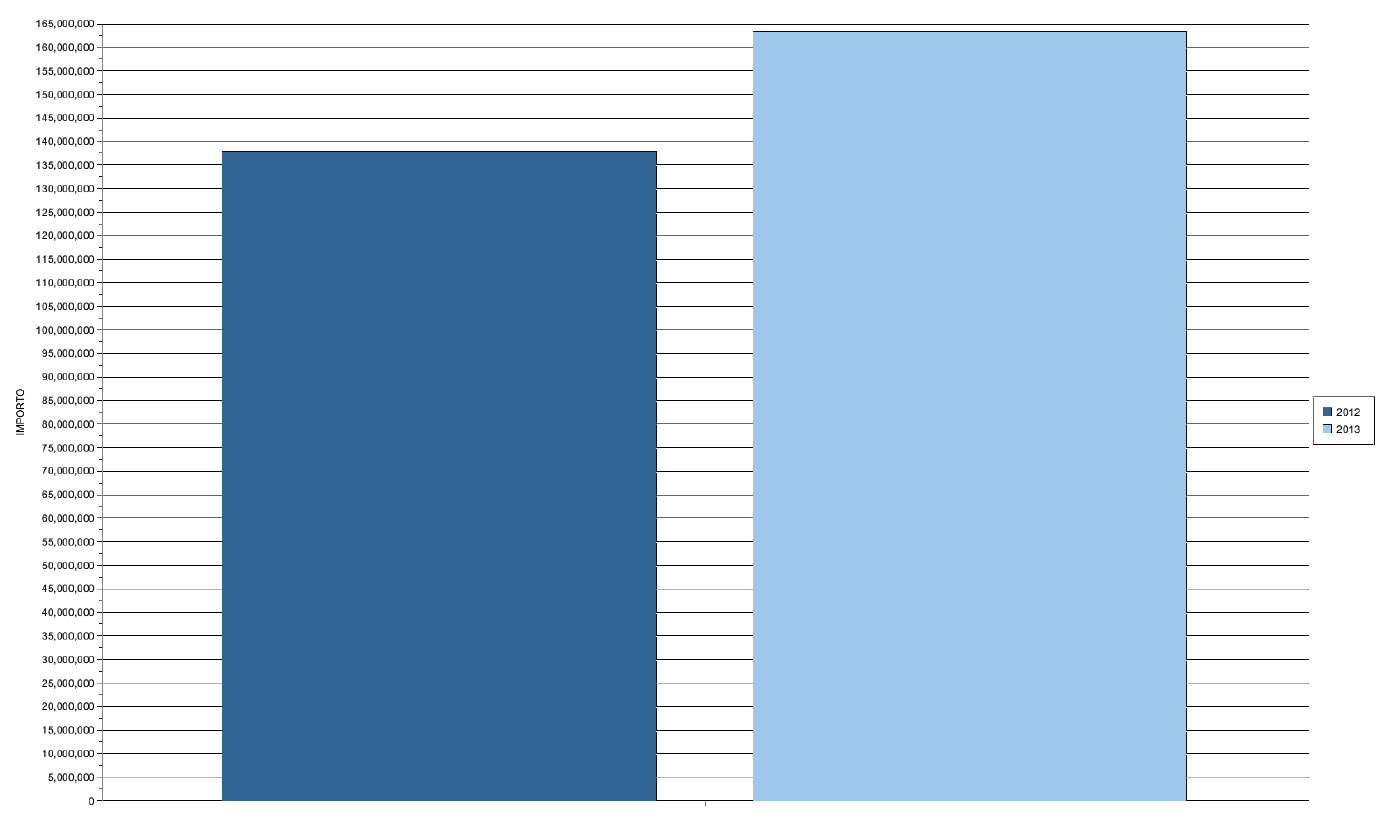
\includegraphics[scale=0.5]{totale_costo.png}
				\caption{Totale Costo 2012/2013, grafico.}
				\label{fig:totale_costo}
			\end{figure}
			
			\begin{figure}[h!]
				\centering
					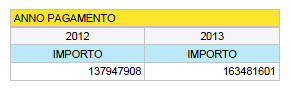
\includegraphics[scale=0.8]{totale_costo_tab.png}
				\caption{Totale Costo 2012/2013, tabella.}
				\label{fig:totale_costo_tab}
			\end{figure}
			
			Nonostante il bilancio 2013 non sia definitivo, vediamo come quest'ultimo superi già il bilancio 2012 in termini di costo di circa 25 milioni di euro. Questa disparità può essere spiegata col fatto che il bilancio 2012 è, a sua volta, non completo, in quanto, come già accennato nel Capitolo \ref{chap:elaborazione}, esso inizia a partire dal 26 giugno 2012.
			
			\FloatBarrier
			
		\subsection{Confronto: Totale Pagamenti/Crediti 2012/2013} \label{subsce:pagamenti/crediti}
		
			In questa analisi partiamo dalla precedente ed entriamo nel dettaglio di Pagamenti e Crediti, disaggregando rispetto al campo \texttt{DOCUMENTO}, che indica se una commissione è una \textit{fattura} o una \textit{nota di credito}.\\
			
			\begin{figure}[h!]
				\centering
					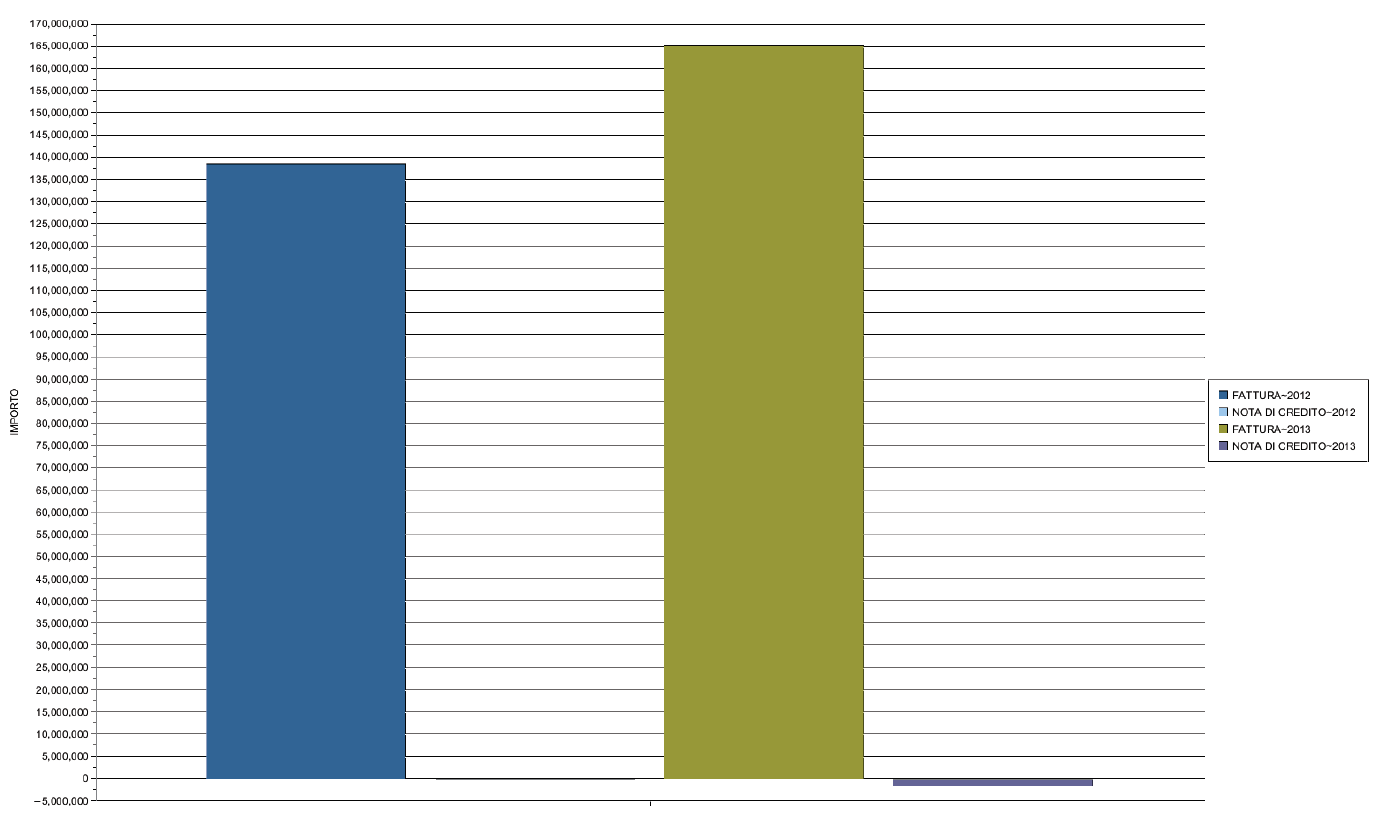
\includegraphics[scale=0.5]{totale_pagamenti-crediti.png}
				\caption{Totale Pagamenti/Crediti 2012/2013, grafico.}
				\label{fig:totale_pagamenti-crediti}
			\end{figure}
			
			\begin{figure}[h!]
				\centering
					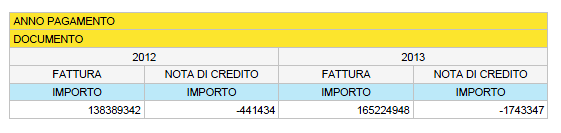
\includegraphics[scale=0.8]{totale_pagamenti-crediti_tab.png}
				\caption{Totale Pagamenti/Crediti 2012/2013, tabella.}
				\label{fig:totale_pagamenti-crediti_tab}
			\end{figure}
			
			Come nel caso precedente, notiamo che il bilancio 2013 presenta valori più alti (in valore assoluto), sia per Pagamenti che per Crediti, probabilmente per la stessa considerazione fatta precedentemente.
			
			\FloatBarrier
			
		\subsection{Confronto: Totale Fatture/Note di Credito 2012/2013} \label{subsec:fatture/notedicredito}
		
			Per avere una conferma delle supposizioni fatte nelle ultime due analisi, andiamo ad osservare quanti mandati sono stati commissionati negli anni 2012/2013, mantenendo la distinzione tra fatture e note di credito.\\
		
			\begin{figure}[h!]
				\centering
					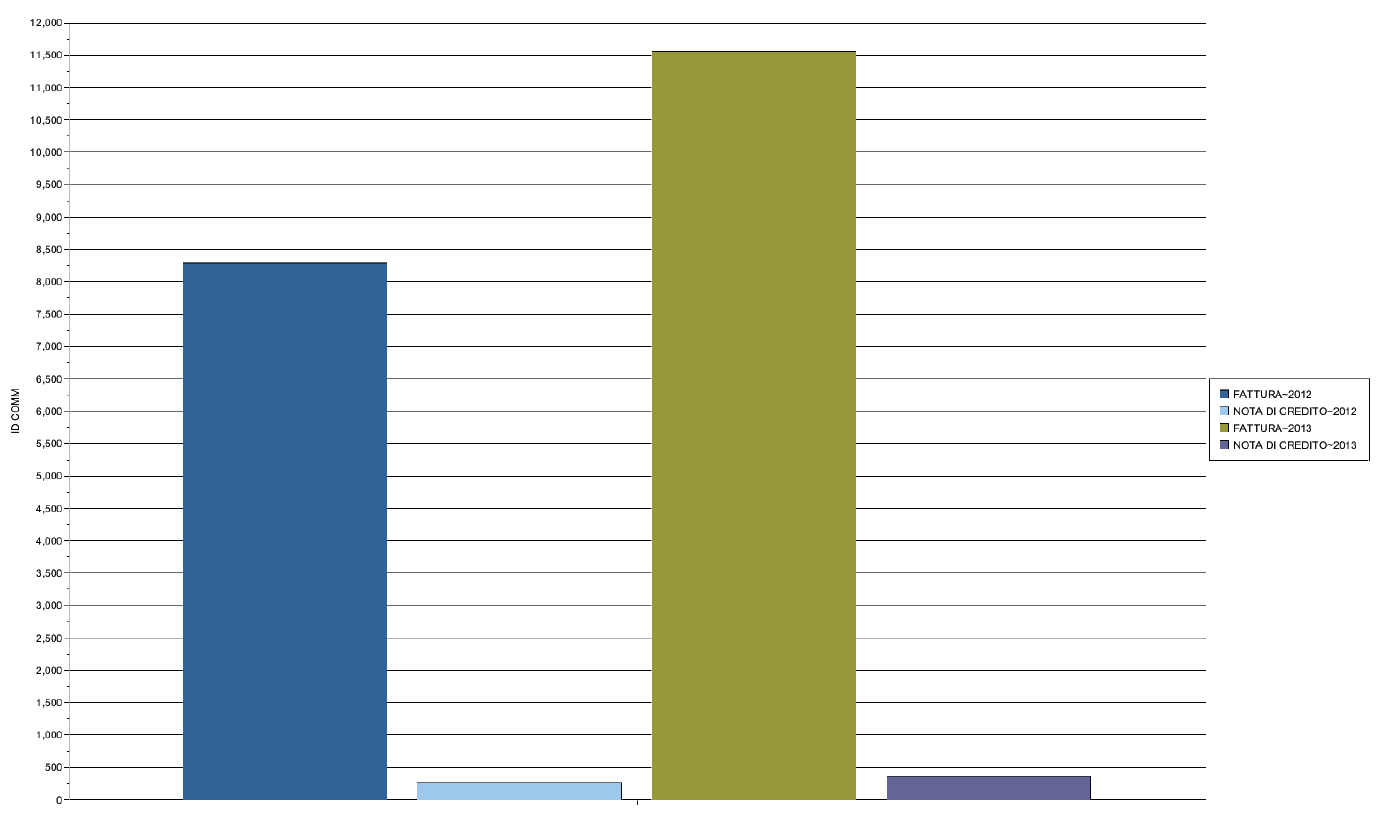
\includegraphics[scale=0.5]{totale_fatture-notedicredito.png}
				\caption{Totale Fatture/Note di Credito 2012/2013, grafico.}
				\label{fig:totale_fatture-notedicredito}
			\end{figure}
			
			\begin{figure}[h!]
				\centering
					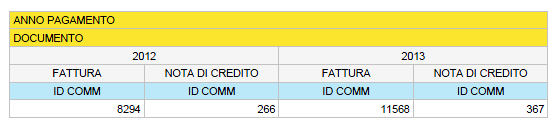
\includegraphics[scale=0.8]{totale_fatture-notedicredito_tab.png}
				\caption{Totale Fatture/Note di Credito 2012/2013, tabella.}
				\label{fig:totale_fatture-notedicredito_tab}
			\end{figure}
			
			Come ci aspettavamo, si nota che nel 2013 sono stati commissionati più lavori (sia a credito che non), probabilmente proprio a causa delle mancanze presenti nel bilancio 2012 prima menzionate.
			
			\FloatBarrier
			
	\section{TOP 10 Pagamenti per Aziende} \label{sec:pagamenti_aziende}
		
		Le analisi di questa sezione saranno orientate ad individuare le Aziende più pagate dal Comune di Firenze: vedremo innanzitutto la Top-10 delle Aziende più pagate nel 2012, quindi nel 2013 ed infine verrano confrontati i pagamenti tra 2012 e 2013 per le Aziende relative alla prima di queste analisi.
		
		\subsection{TOP 10 Pagamenti per Aziende 2012} \label{subsec:pagamenti_aziende_2012}
		
			Vediamo in questa analisi quali sono state le 10 Aziende più pagate dal Comune di Firenze durante l'anno 2012.\\
			
			\begin{figure}[h!]
				\centering
					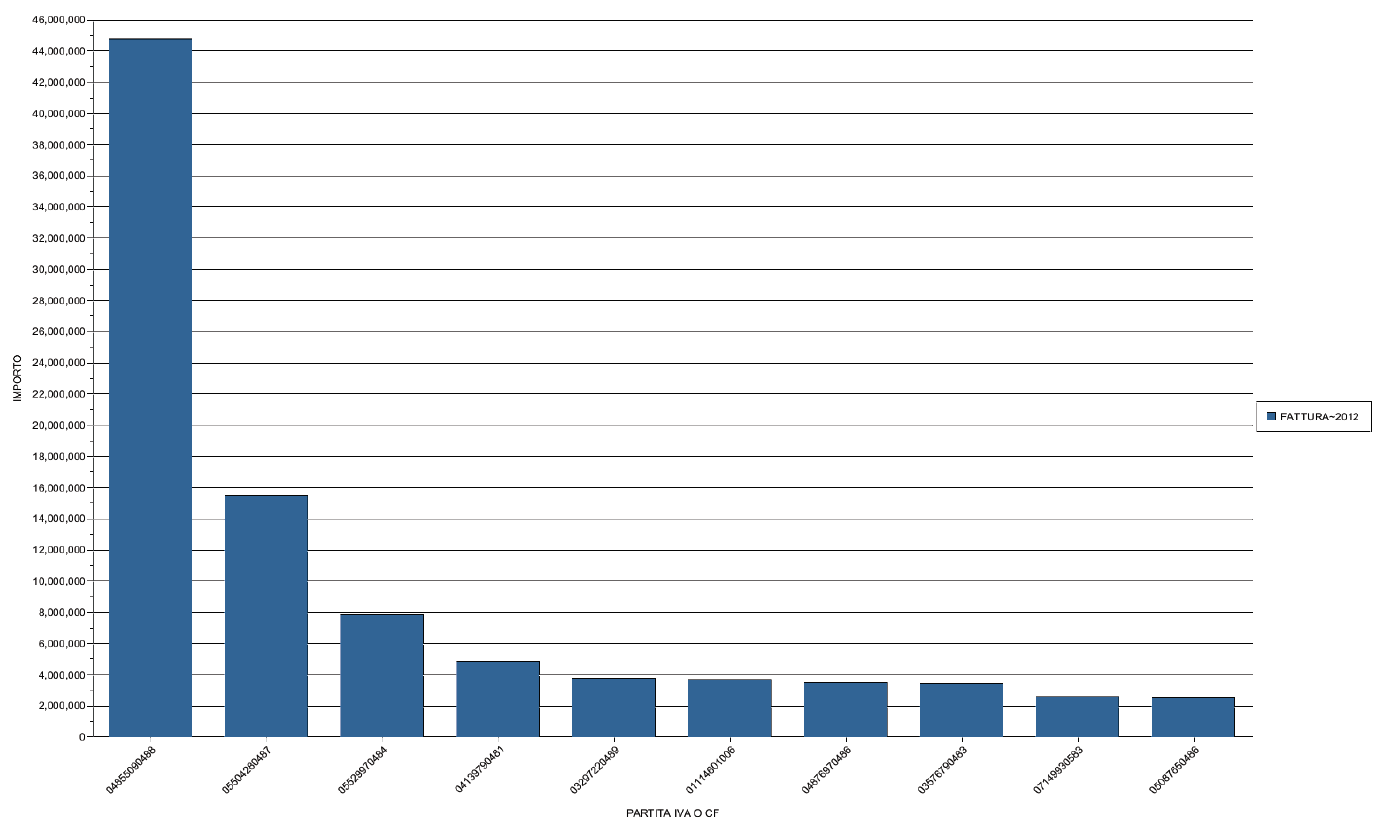
\includegraphics[scale=0.5]{top10_pagamenti_aziende_2012.png}
				\caption{TOP 10 Pagamenti per Aziende 2012, grafico.}
				\label{fig:top10_pagamenti_aziende_2012}
			\end{figure}
			
			\begin{figure}[h!]
				\centering
					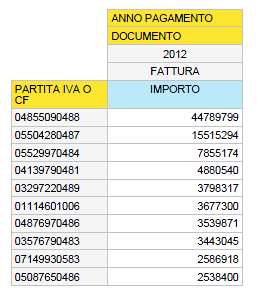
\includegraphics[scale=0.8]{top10_pagamenti_aziende_2012_tab.png}
				\caption{TOP 10 Pagamenti per Aziende 2012, tabella.}
				\label{fig:top10_pagamenti_aziende_2012_tab}
			\end{figure}
			
			\begin{figure}[h!]
				\centering
					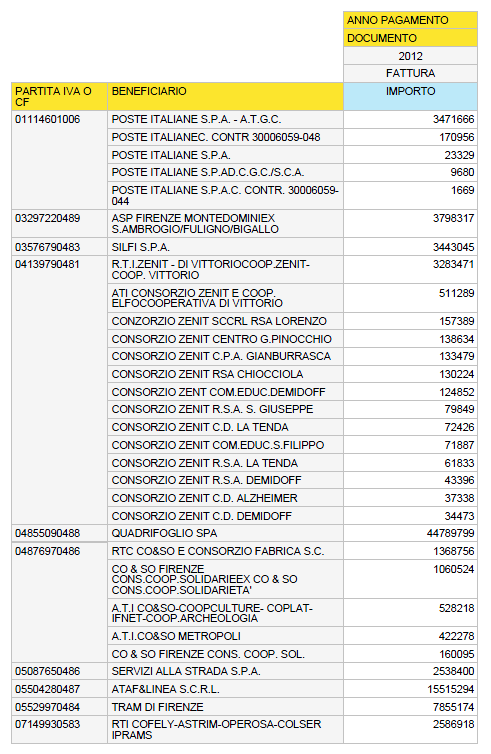
\includegraphics[scale=0.8]{top10_pagamenti_aziende_2012_tab_dis.png}
				\caption{TOP 10 Pagamenti per Aziende 2012, tabella disaggregata.}
				\label{fig:top10_pagamenti_aziende_2012_tab_dis}
			\end{figure}
			
			Si nota subito l'enorme disparità che intercorre tra la prima Azienda, ovvero la \textit{Quadrifoglio s.p.a.}, e tutte le altre presenti nella Top-10.\\
			La \textit{Quadrifoglio s.p.a.} è un'Azienda di Firenze che si occupa di servizi ambientali nel Comune di Firenze e nei comuni limitrofi, offrendo servizi come raccolta e smaltimento rifiuti, in primo luogo, ma anche come disinfestazione (zanzare, topi, ecc\dots) o centro di analisi e ricerca. È quindi un'Azienda molto importante, ormai onnipresente nell'ambiente fiorentino, che giustifica tutte le spese osservate.\\
			Com'è facile aspettarsi, al secondo e terzo posto troviamo altre due Aziende onnipresenti nello senario fiorentino: \textit{ATAF\&Linea S.C.R.L.} e \textit{Tram di Firenze}, che si occupano, rispettivamente, del servizio di autobus e della tramvia fiorentina.
			Tra le altre Aziende, troviamo altri nomi ben conosciuti come \textit{Consorzio Zenit}, che si occupa di interventi educativi, formativi e sanitari, e le \textit{Poste Italiane}.
			
			\FloatBarrier
		
		\subsection{TOP 10 Pagamenti per Aziende 2013} \label{subsec:pagamenti_aziende_2013}
		
			Ripetiamo qui l'analisi precedente sull'anno 2013 anziché 2012.\\
		
			\begin{figure}[h!]
				\centering
					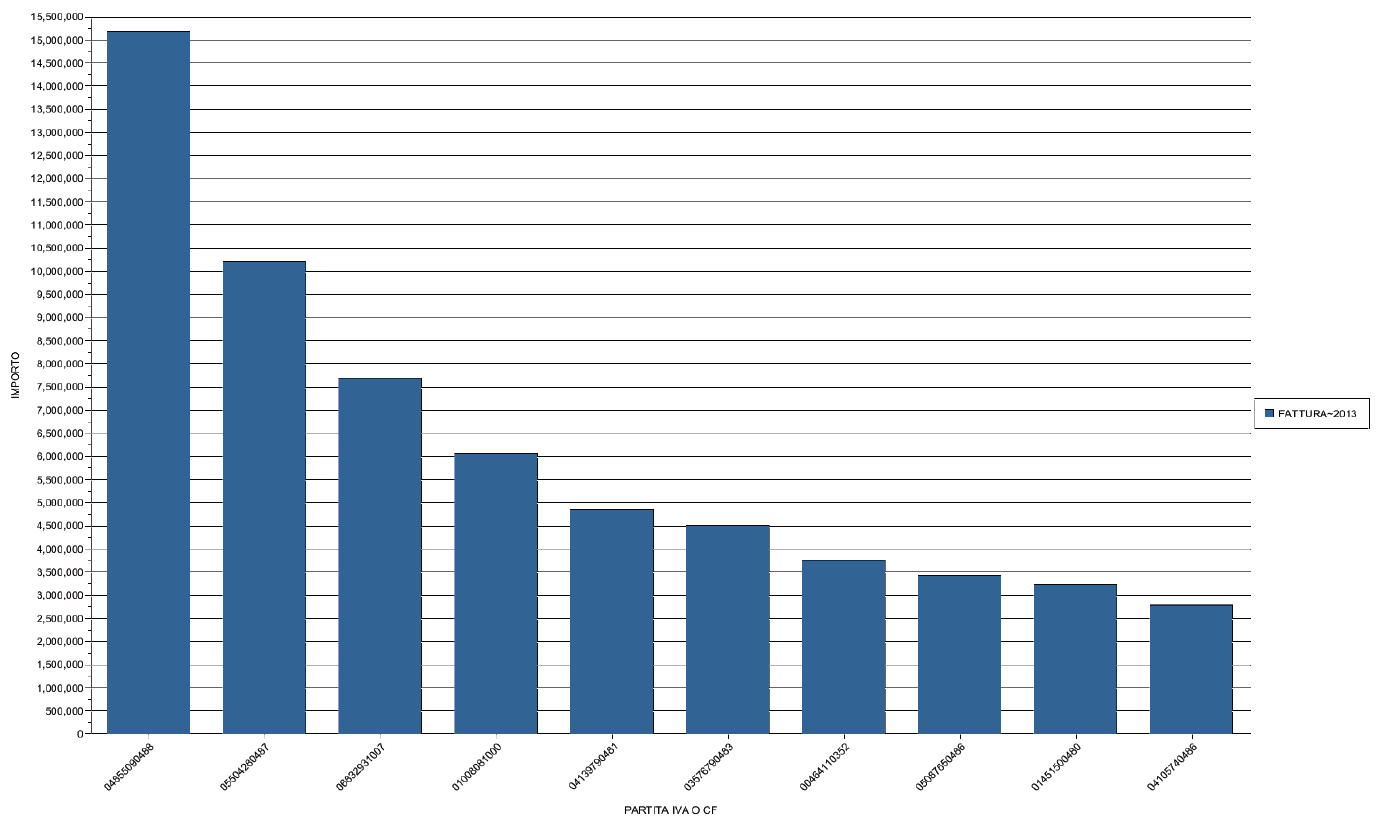
\includegraphics[scale=0.5]{top10_pagamenti_aziende_2013.png}
				\caption{TOP 10 Pagamenti per Aziende 2013, grafico.}
				\label{fig:top10_pagamenti_aziende_2013}
			\end{figure}
			
			\begin{figure}[h!]
				\centering
					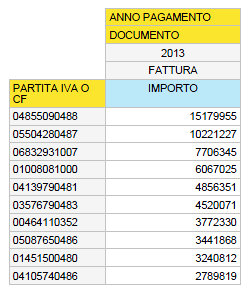
\includegraphics[scale=0.8]{top10_pagamenti_aziende_2013_tab.png}
				\caption{TOP 10 Pagamenti per Aziende 2013, tabella.}
				\label{fig:top10_pagamenti_aziende_2013_tab}
			\end{figure}
			
			\begin{figure}[h!]
				\centering
					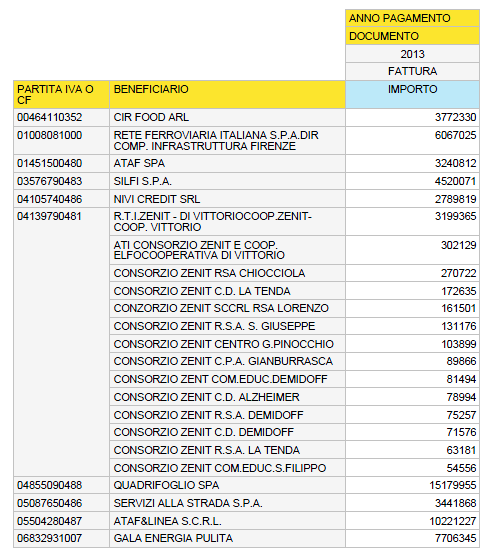
\includegraphics[scale=0.8]{top10_pagamenti_aziende_2013_tab_dis.png}
				\caption{TOP 10 Pagamenti per Aziende 2013, tabella disaggregata.}
				\label{fig:top10_pagamenti_aziende_2013_tab_dis}
			\end{figure}
			
			Al primo e secondo posto troviamo ancora la \textit{Quadrifoglio s.p.a.} e \textit{ATAF\&Linea S.C.R.L.}, esattamente come nel 2012. Al terzo posto troviamo invece \textit{Gala Energia Pulita}, che si occupa di fornitura energetica. Tra le altre, ritroviamo il \textit{Consorzio Zenit} ed altre Aziende.
			
			\FloatBarrier
		
		\subsection{Confronto: TOP 10 Pagamenti per Aziende 2012/2013} \label{subsec:pagamenti_aziende_2012/2013}
	
			Vediamo adesso come le Aziende presenti nella Top-10 di Pagamenti del 2012 vengono pagate tra il 2012 ed il 2013.\\
	
			\begin{figure}[h!]
				\centering
					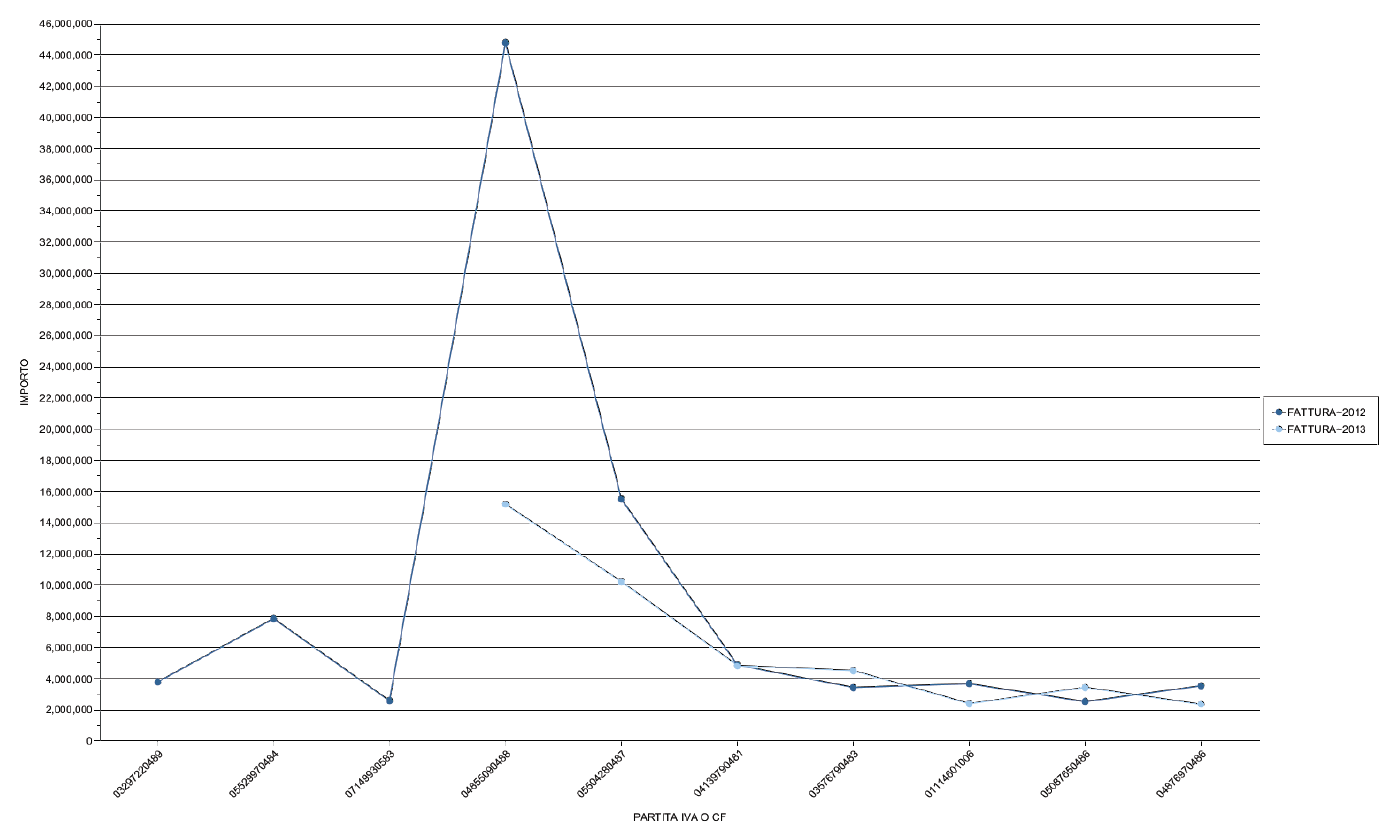
\includegraphics[scale=0.5]{top10_pagamenti_aziende_2012-2013.png}
				\caption{TOP 10 Pagamenti per Aziende 2012/2013, grafico.}
				\label{fig:top10_pagamenti_aziende_2012-2013}
			\end{figure}
			
			\begin{figure}[h!]
				\centering
					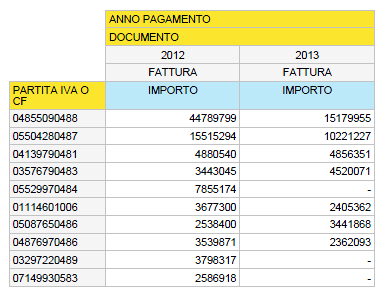
\includegraphics[scale=0.8]{top10_pagamenti_aziende_2012-2013_tab.png}
				\caption{TOP 10 Pagamenti per Aziende 2012/2013, tabella.}
				\label{fig:top10_pagamenti_aziende_2012-2013_tab}
			\end{figure}
			
			\begin{figure}[h!]
				\centering
					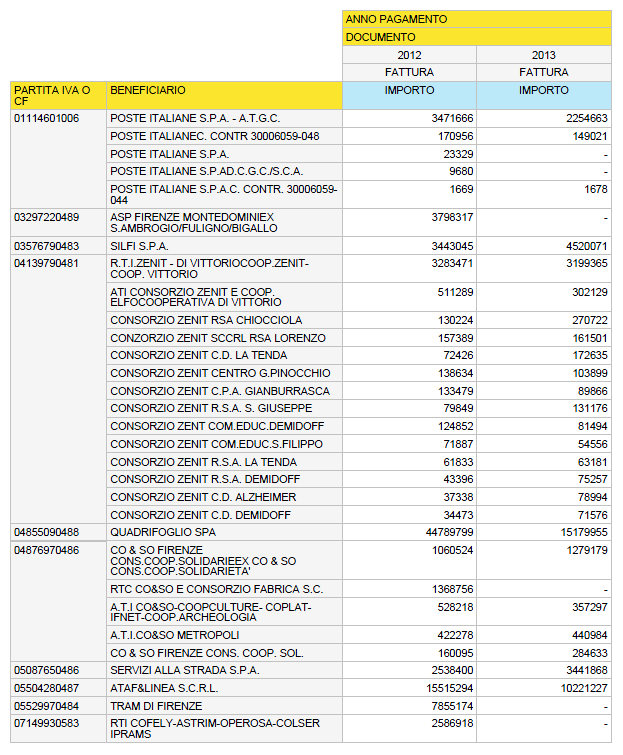
\includegraphics[scale=0.8]{top10_pagamenti_aziende_2012-2013_tab_dis.png}
				\caption{TOP 10 Pagamenti per Aziende 2012/2013, tabella disaggregata.}
				\label{fig:top10_pagamenti_aziende_2012-2013_tab_dis}
			\end{figure}
			
			Si notano innanzitutto tre aziende (\textit{Tram di Firenze}, \textit{RTI Cofely-Astrim-Operosa-Colser Iprams} e \textit{ASP Firenze Montedomini}) presenti nella Top-10 2012 e del tutto assenti nel bilancio 2013, indice, probabilmente, di Aziende a cui erano stati assegnati lavori una tantum. Si nota inoltre la disparità dei pagamenti verso \textit{Quadrifoglio s.p.a.} che, nonostante sia comunque la più pagata delle Aziende, ha registrato comunque un forte crollo rispetto al 2012. Per quanto riguarda le altre Aziende, si registra invece un andamento piuttosto regolare nel biennio 2012/2013.
			
			\FloatBarrier
	
	\section{TOP 10 Pagamenti per Direzioni} \label{sec:top_pagamenti_direzioni}
	
		Dal momento che le Direzioni di Servizio sono delle classificazioni per area di competenza del Comune di Firenze, possiamo vedere i pagamenti approvati da una certa Direzione come gli investimenti del Comune nelle rispettive aree.\\
		\\
		Eseguiamo in questa sezione le stesse analisi effettuate in Sezione \ref{sec:pagamenti_aziende}, con l'unica differenza che i pagamenti saranno aggregati per Direzione di Servizio e non più per Azienda. Potremo analizzare in questo modo in quali aree ha scelto di investire il Comune di Firenze e come queste scelte si siano evolute tra il 2012 ed il 2013.
	
		\subsection{TOP 10 Pagamenti per Direzioni 2012} \label{subsec:top_pagamenti_direzioni_2012}
		
			La prima analisi da effettuare è relativa alle 10 Direzioni di Servizio che, nel 2012, hanno pagato di più rispetto alle altre.
		
			\begin{figure}[h!]
				\centering
					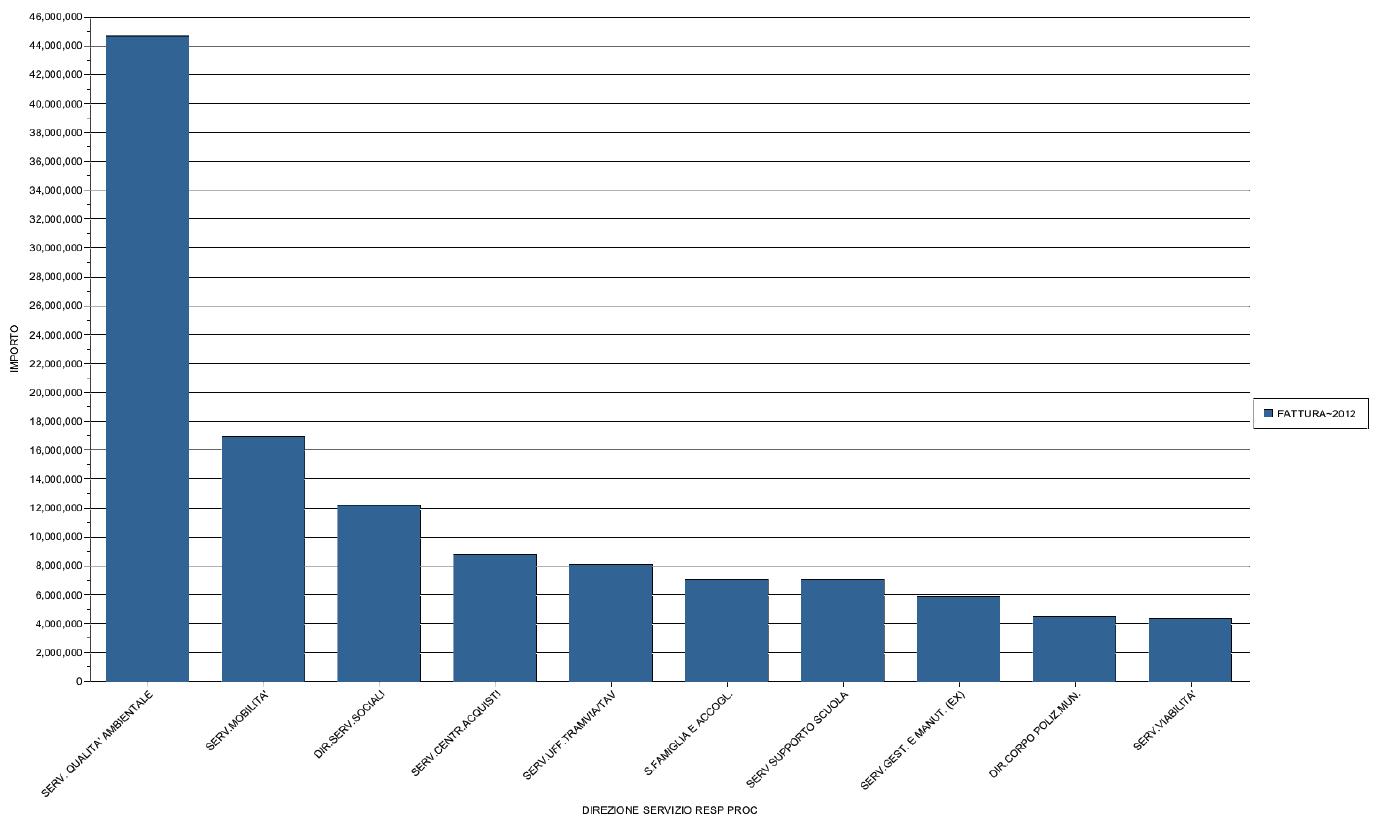
\includegraphics[scale=0.5]{top10_pagamenti_direzioni_2012.png}
				\caption{TOP 10 Pagamenti per Direzioni 2012, grafico.}
				\label{fig:top10_pagamenti_direzioni_2012}
			\end{figure}
			
			\begin{figure}[h!]
				\centering
					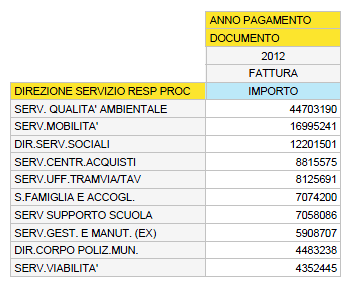
\includegraphics[scale=0.8]{top10_pagamenti_direzioni_2012_tab.png}
				\caption{TOP 10 Pagamenti per Direzioni 2012, tabella.}
				\label{fig:top10_pagamenti_direzioni_2012_tab}
			\end{figure}
			
			Come era intuibile, le Direzioni ad aver speso di più nel 2012 sono \textit{Servizi Qualità Ambientale} e \textit{Servizi Mobilità} (ricordando dalle analisi in Sezione \ref{sec:pagamenti_aziende} che le aziende più pagate nel 2012 erano la \textit{Quadrifoglio s.p.a.}, \textit{Ataf} e \textit{Tram di Firenze}). Tra le altre Direzioni presenti nella Top-10 troviamo altri settori molto importanti, come \textit{Servizi Supporto Scuola}, \textit{Direzione Corpo Polizia Municipale} e \textit{Servizi Viabilità}.
			
			\FloatBarrier
		
		\subsection{TOP 10 Pagamenti per Direzioni 2013} \label{subsec:top_pagamenti_direzioni_2013}
		
			Ripetiamo adesso le analisi per l'anno 2013.
			
			\begin{figure}[h!]
				\centering
					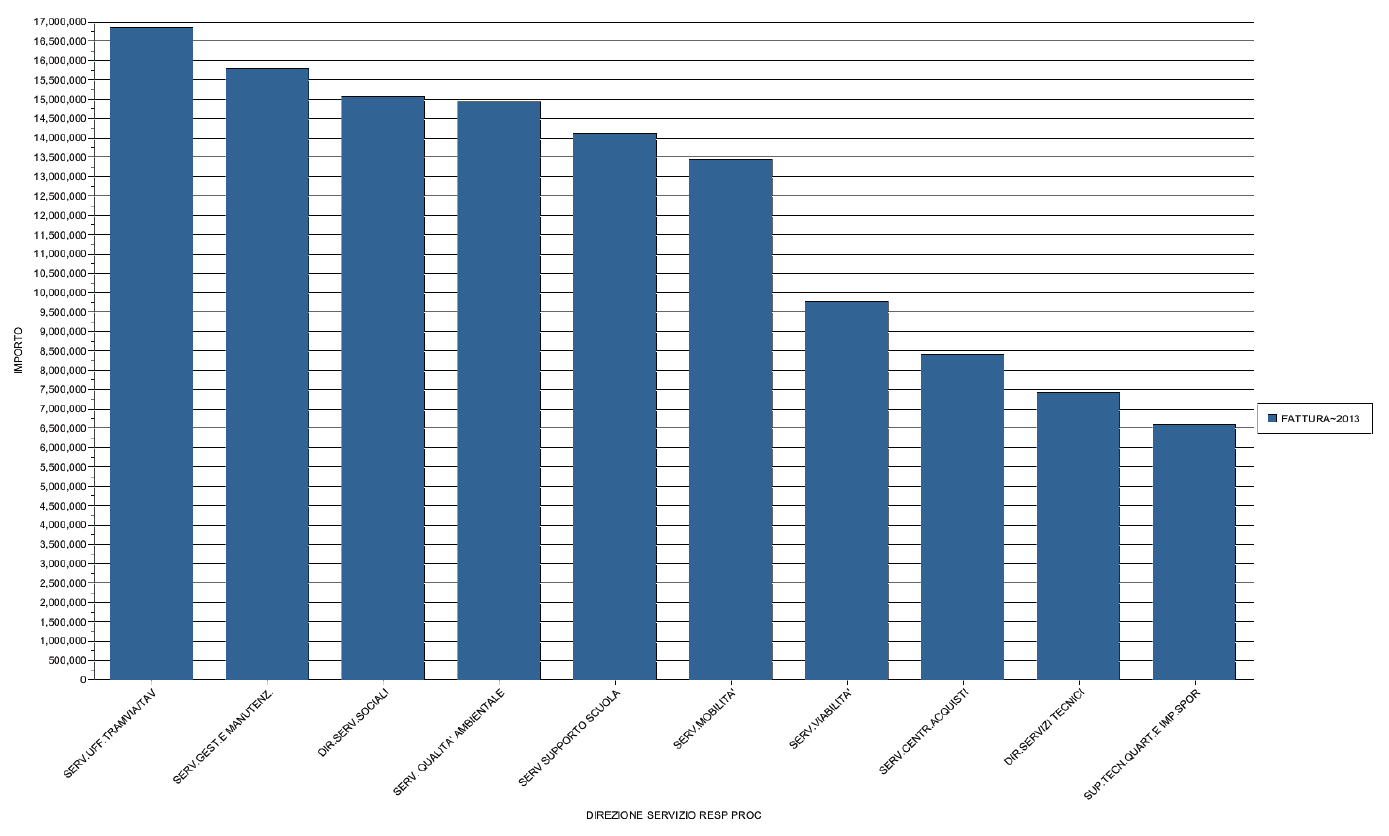
\includegraphics[scale=0.5]{top10_pagamenti_direzioni_2013.png}
				\caption{TOP 10 Pagamenti per Direzioni 2013, grafico.}
				\label{fig:top10_pagamenti_direzioni_2013}
			\end{figure}
			
			\begin{figure}[h!]
				\centering
					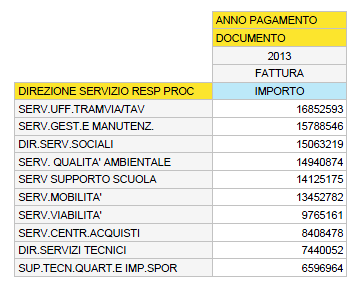
\includegraphics[scale=0.8]{top10_pagamenti_direzioni_2013_tab.png}
				\caption{TOP 10 Pagamenti per Direzioni 2013, tabella.}
				\label{fig:top10_pagamenti_direzioni_2013_tab}
			\end{figure}
			
			Vediamo in questo grafico (Figura \ref{fig:top10_pagamenti_direzioni_2013} che gli importi pagati dalle prima 10 Direzioni nel 2013 sono piuttosto regolari, senza sbalzi o irregolarità troppo evidenti. Rispetto al 2012, gli investimenti sono stati indirizzati più o meno nelle stesse direzioni.
			
			\FloatBarrier
		
		\subsection{Confronto: TOP 10 Pagamenti per Direzioni 2012/2013} \label{subsec:pagamenti_direzioni_2012/2013}
	
			Confrontiamo adesso le Direzioni con più investimenti nel 2012 con gli investimenti nel 2013 (relativamente alle stesse Direzioni di Servizio).
	
			\begin{figure}[h!]
				\centering
					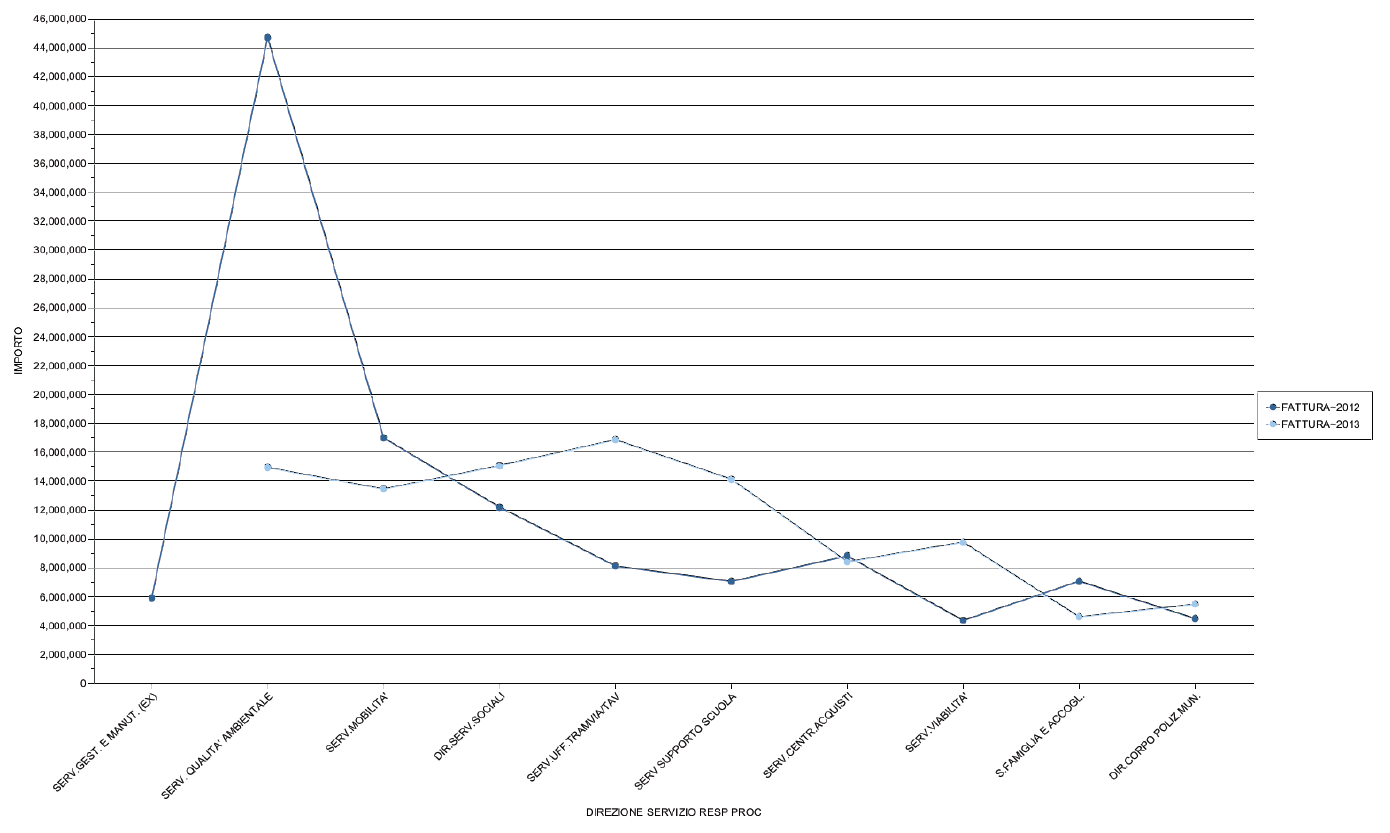
\includegraphics[scale=0.5]{top10_pagamenti_direzioni_2012-2013.png}
				\caption{TOP 10 Pagamenti per Direzioni 2012/2013, grafico.}
				\label{fig:top10_pagamenti_direzioni_2012-2013}
			\end{figure}
			
			\begin{figure}[h!]
				\centering
					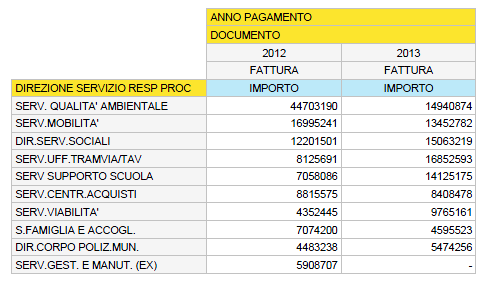
\includegraphics[scale=0.8]{top10_pagamenti_direzioni_2012-2013_tab.png}
				\caption{TOP 10 Pagamenti per Direzioni 2012/2013, tabella.}
				\label{fig:top10_pagamenti_direzioni_2012-2013_tab}
			\end{figure}
			
			A parte \textit{Servizi Gestione e Manutenzione}, che non è presente nel bilancio 2013, notiamo nel grafico in Figura \ref{fig:top10_pagamenti_direzioni_2012-2013} un netto distacco nei finanziamenti 2012 e 2013. Il cambiamento più eclatante risulta essere quello relativo ai \textit{Servizi Qualità Ambientale}, in accordo con quanto osservato in Sezione \ref{sec:pagamenti_aziende}, che registra un calo di quasi 30 milioni di euro negli investimenti, pari a circa $66\%$ degli investimenti registrati nel 2012.
			
			\FloatBarrier
	
	\section{BOTTOM 10 Pagamenti per Direzioni} \label{sec:bottom_pagamenti_direzioni}
	
		Avendo osservato le Direzioni con più investimenti, analizziamo in questa sezione le aree con meno investimenti.
	
		\subsection{BOTTOM 10 Pagamenti per Direzioni 2012} \label{subsec:bottom_pagamenti_direzioni_2012}
		
			Questa analisi rappresenta la Bottom-10 degli investimenti nel 2012, ovvero le 10 Direzioni di Servizio del Comune di Firenze che hanno speso meno nell'anno 2012.
		
			\begin{figure}[h!]
				\centering
					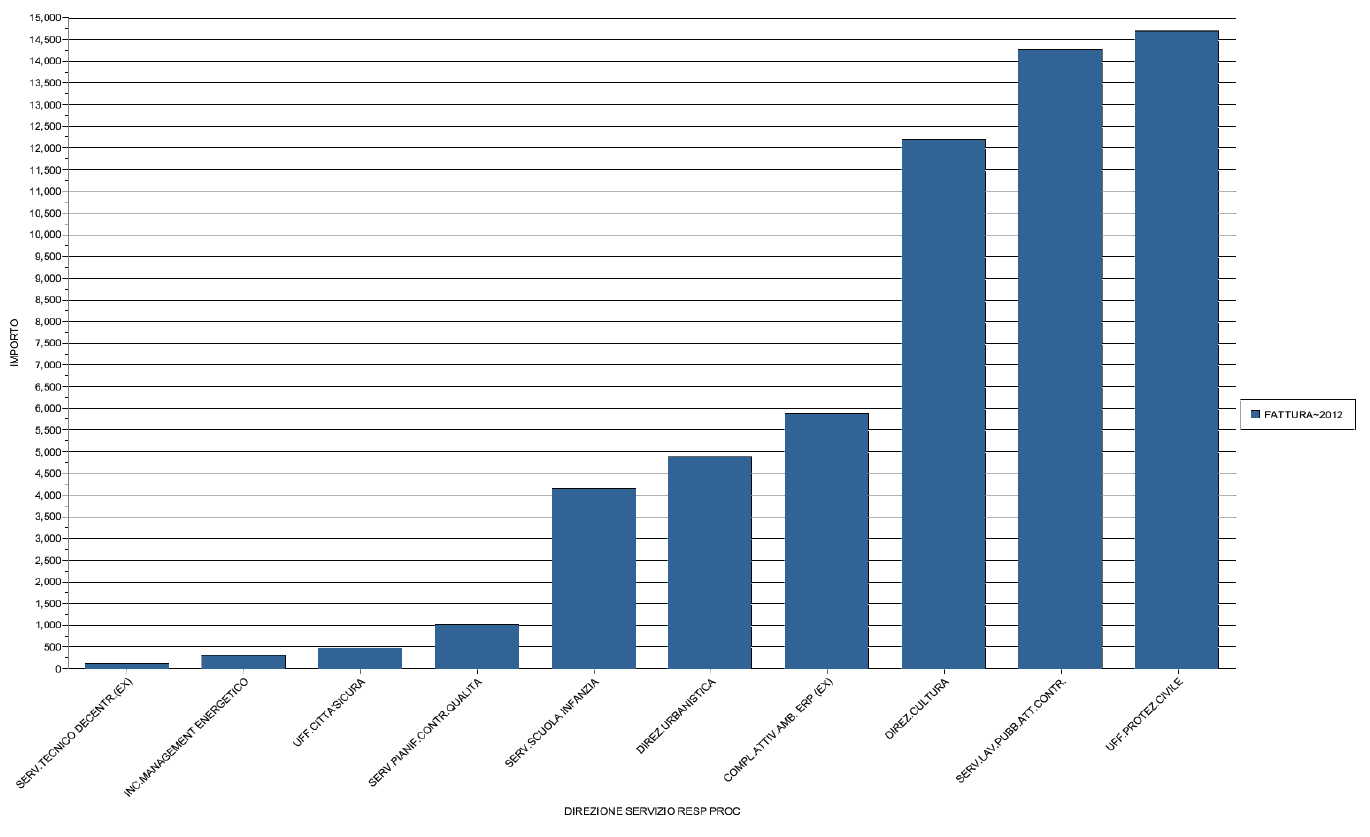
\includegraphics[scale=0.5]{bottom10_pagamenti_direzioni_2012.png}
				\caption{BOTTOM 10 Pagamenti per Direzioni 2012, grafico.}
				\label{fig:bottom10_pagamenti_direzioni_2012}
			\end{figure}
			
			\begin{figure}[h!]
				\centering
					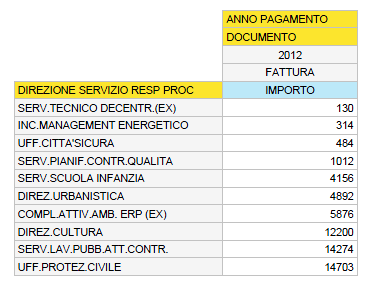
\includegraphics[scale=0.8]{bottom10_pagamenti_direzioni_2012_tab.png}
				\caption{BOTTOM 10 Pagamenti per Direzioni 2012, tabella.}
				\label{fig:bottom10_pagamenti_direzioni_2012_tab}
			\end{figure}
			
			Osservando il grafico di quest'analisi, si può vedere come alcuni importanti settori, come \textit{Protezione Civile}, \textit{Cultura} o \textit{Scuola dell'Infanzia}, siano stati alquanto trascurate per quanto riguarda gli investimenti promossi dal Comune di Firenze. Anche se si tratta, senza dubbio, di aree molto importanti, quella con più investimenti tra le 10 in questione registra poco più di 14mila euro di investimenti, mentre la prima registra soltanto 130 euro.
			
			\FloatBarrier
		
		\subsection{BOTTOM 10 Pagamenti per Direzioni 2013} \label{subsec:bottom_pagamenti_direzioni_2013}
		
			Analizziamo adesso gli investimenti più bassi nel 2013.
		
			\begin{figure}[h!]
				\centering
					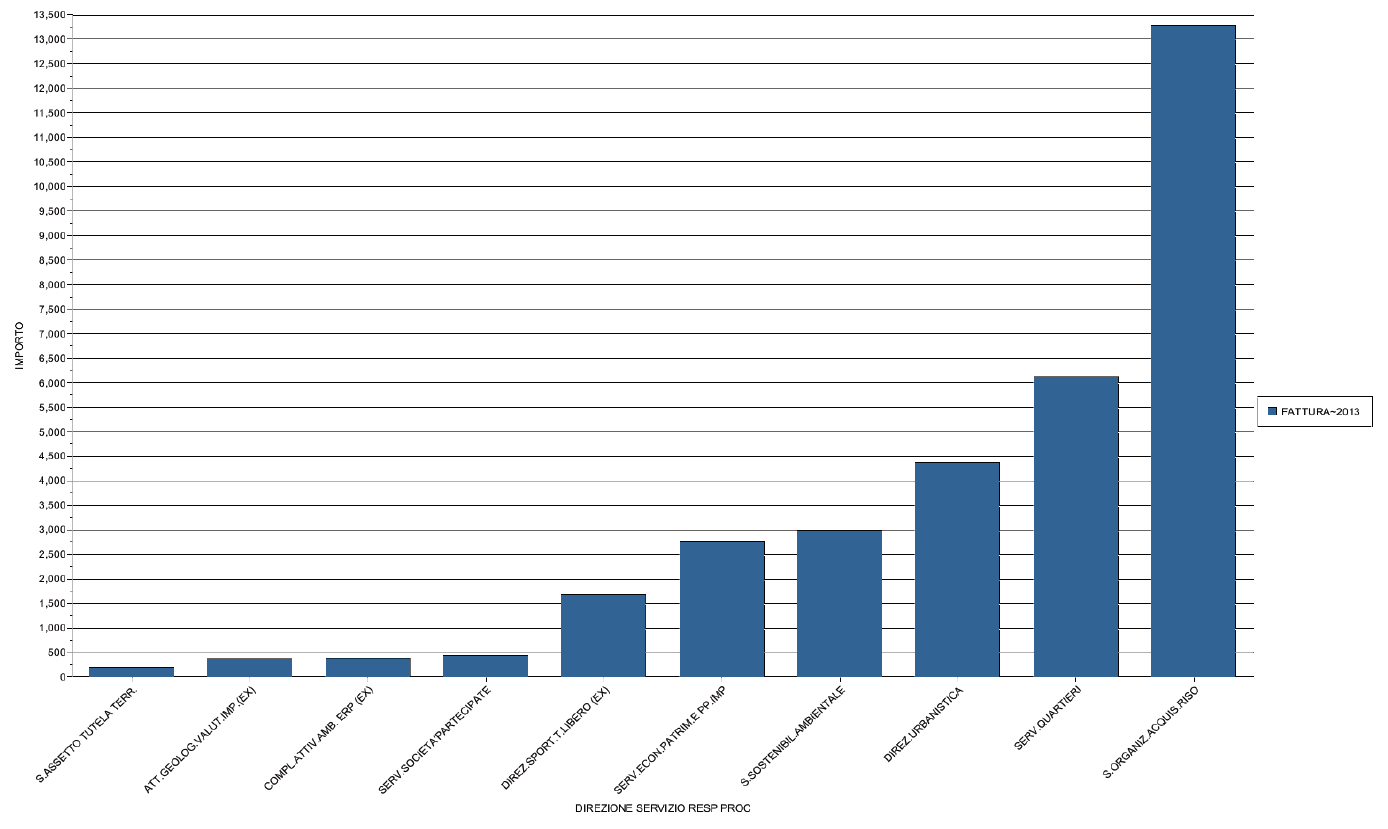
\includegraphics[scale=0.5]{bottom10_pagamenti_direzioni_2013.png}
				\caption{BOTTOM 10 Pagamenti per Direzioni 2013, grafico.}
				\label{fig:bottom10_pagamenti_direzioni_2013}
			\end{figure}
			
			\begin{figure}[h!]
				\centering
					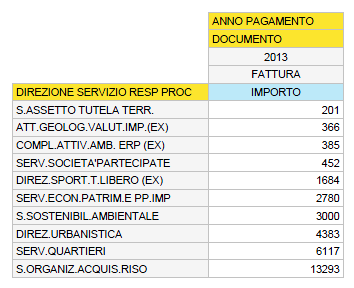
\includegraphics[scale=0.8]{bottom10_pagamenti_direzioni_2013_tab.png}
				\caption{BOTTOM 10 Pagamenti per Direzioni 2013, tabella.}
				\label{fig:bottom10_pagamenti_direzioni_2013_tab}
			\end{figure}
			
			Fortunatamente, dal grafico e dalla tabella risulta che durante il 2013 gli investimenti più bassi del Comune di Firenze sono relativi a settori ed aree minori, che giustificano i bassi costi riscontrati.
			
			\FloatBarrier
		
		\subsection{Confronto: BOTTOM 10 Pagamenti per Direzioni 2012/2013} \label{subsec:bottom_pagamenti_direzioni_2012/2013}
	
			Confrontiamo adesso le Direzioni che hanno pagato di meno nel 2012, mostrando la loro evoluzione tra il 2012 ed il 2013.
	
			\begin{figure}[h!]
				\centering
					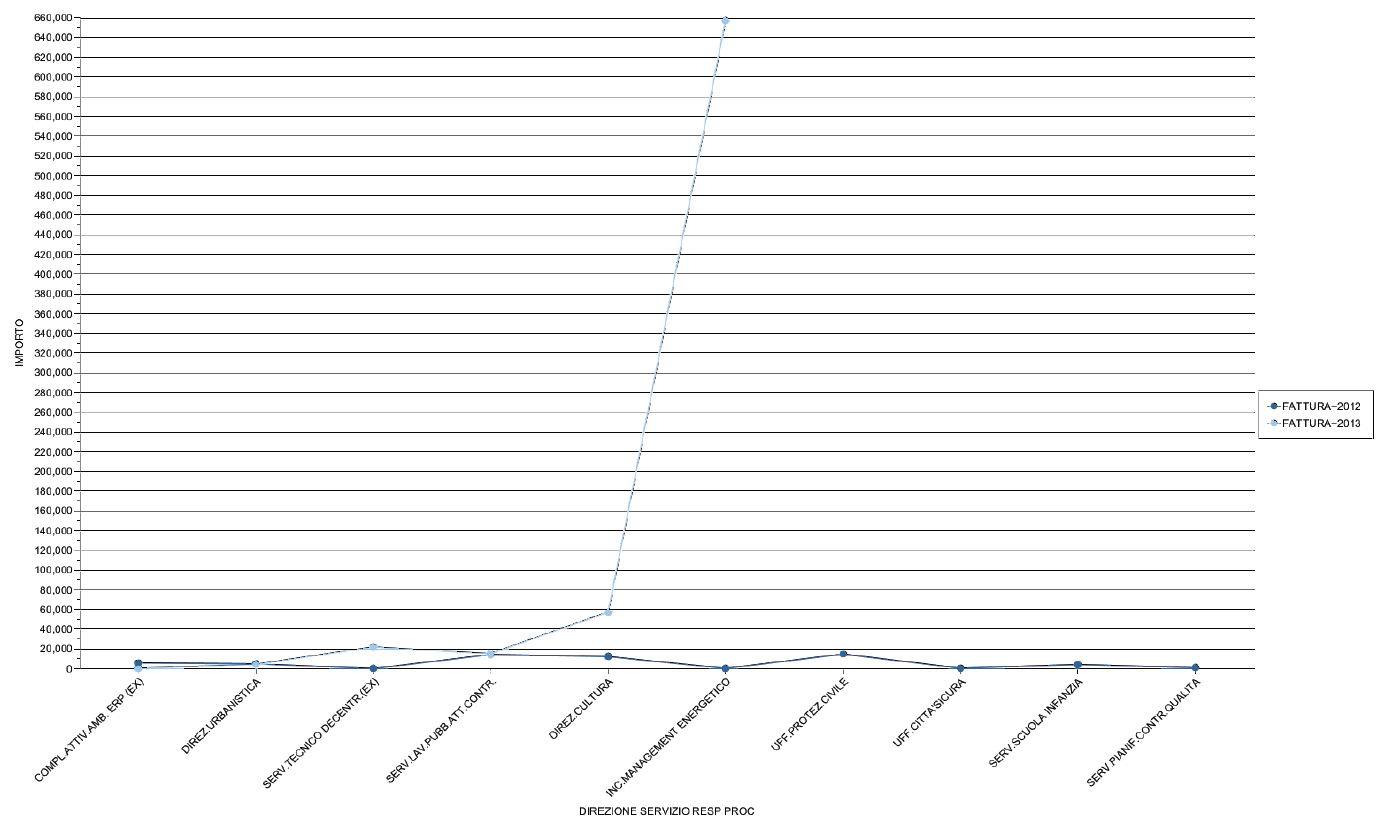
\includegraphics[scale=0.5]{bottom10_pagamenti_direzioni_2012-2013.png}
				\caption{BOTTOM 10 Pagamenti per Direzioni 2012/2013, grafico.}
				\label{fig:bottom10_pagamenti_direzioni_2012-2013}
			\end{figure}
			
			\begin{figure}[h!]
				\centering
					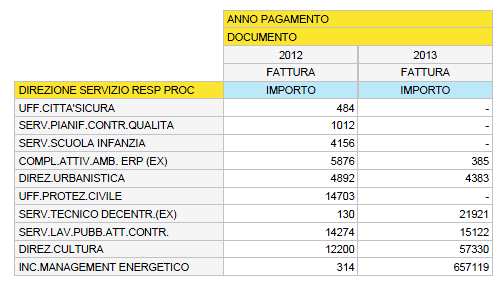
\includegraphics[scale=0.8]{bottom10_pagamenti_direzioni_2012-2013_tab.png}
				\caption{BOTTOM 10 Pagamenti per Direzioni 2012/2013, tabella.}
				\label{fig:bottom10_pagamenti_direzioni_2012-2013_tab}
			\end{figure}
			
			La cosa che risalta subito all'occhio è l'enorme distacco presente negli investimenti nel settore \textit{Management Energetico}, che registra un sostanziale aumento di finanziamenti nel 2013 rispetto al 2012. Inoltre si nota anche un aumento degli investimenti di circa il $369\%$ per quanto riguarda il settore della \textit{Cultura}.\\
			Per quanto riguarda le altre Direzioni, o esse sono assenti nel bilancio 2013, o gli investimenti risultano essere più o meno gli stessi del 2012.
			
			\FloatBarrier
	
	\section{TOP 10 Accoppiate Direzione-Azienda} \label{sec:accoppiate}
		
		Proponiamo in questa sezione un'analisi piuttosto interessante: vogliamo ottenere la lista delle 10 accoppiate Azienda-Direzione di Servizio più frequenti nel biennio 2012/2013.
		
		\begin{figure}[h!]
			\centering
				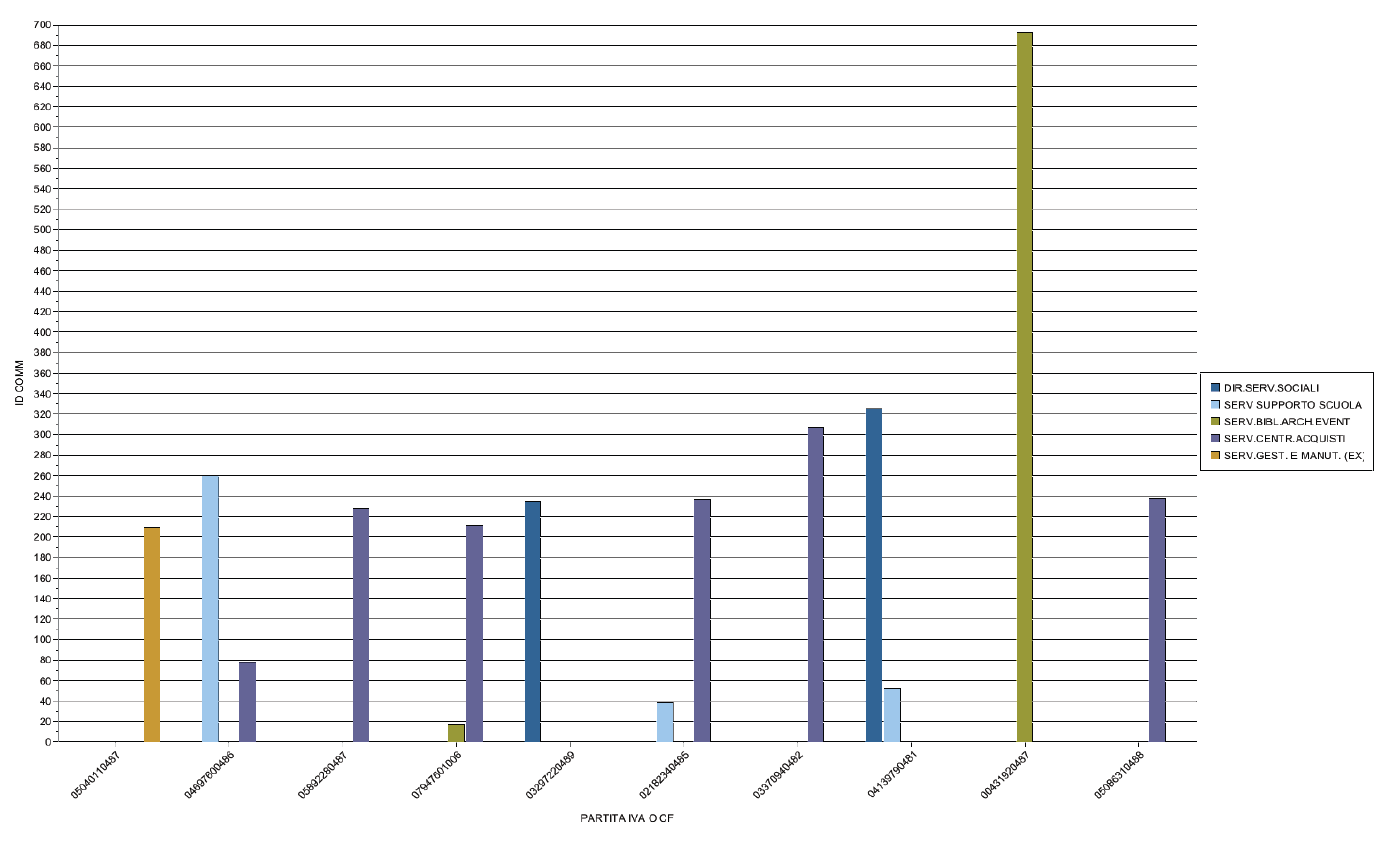
\includegraphics[scale=0.5]{top10_accoppiate.png}
			\caption{TOP 10 Accoppiate Direzione-Azienda, grafico.}
			\label{fig:top10_accoppiate}
		\end{figure}
		
		\begin{figure}[h!]
			\centering
				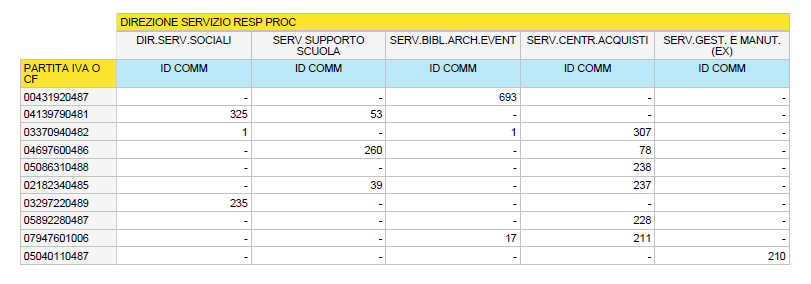
\includegraphics[scale=0.8]{top10_accoppiate_tab.png}
			\caption{TOP 10 Accoppiate Direzione-Azienda, tabella.}
			\label{fig:top10_accoppiate_tab}
		\end{figure}
		
		\begin{figure}[h!]
			\centering
				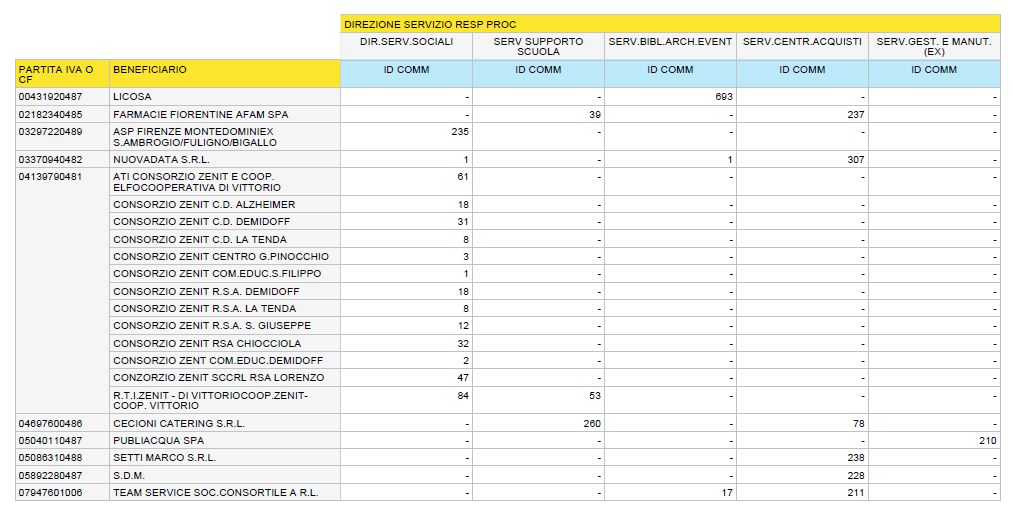
\includegraphics[scale=0.8]{top10_accoppiate_tab_dis.png}
			\caption{TOP 10 Accoppiate Direzione-Azienda, tabella disaggregata.}
			\label{fig:top10_accoppiate_tab_dis}
		\end{figure}
		
		Al primo posto, con ben 693 commissioni, troviamo la Direzione \textit{Servizi Biblioteche e Archivistica} e l'Azienda \textit{Licosa}. \textit{Licosa} è infatti un'Azienda fiorentina che si occupa di abbonamenti a riviste, fornitura e ricerca di libri e pubblicazioni.\\
		Al secondo posto troviamo invece la coppia \textit{Direzione Servizi Sociali} con il \textit{Consorzio Zenit} (che avevamo già citato in Sezione \ref{sec:pagamenti_aziende} tra le Aziende più pagate nel 2012/2013).
		
		\FloatBarrier
	
	\section{TOP 10 Anni di Pagamento per Aziende} \label{sec:anni_pagamento_aziende}
		
		Adesso ci proponiamo invece di individuare a quali Aziende, tra quelle presenti nei bilanci 2012/2013, sono stati assegnati i lavori più lunghi (e presumibilmente più impegnativi).
		
		\begin{figure}[h!]
			\centering
				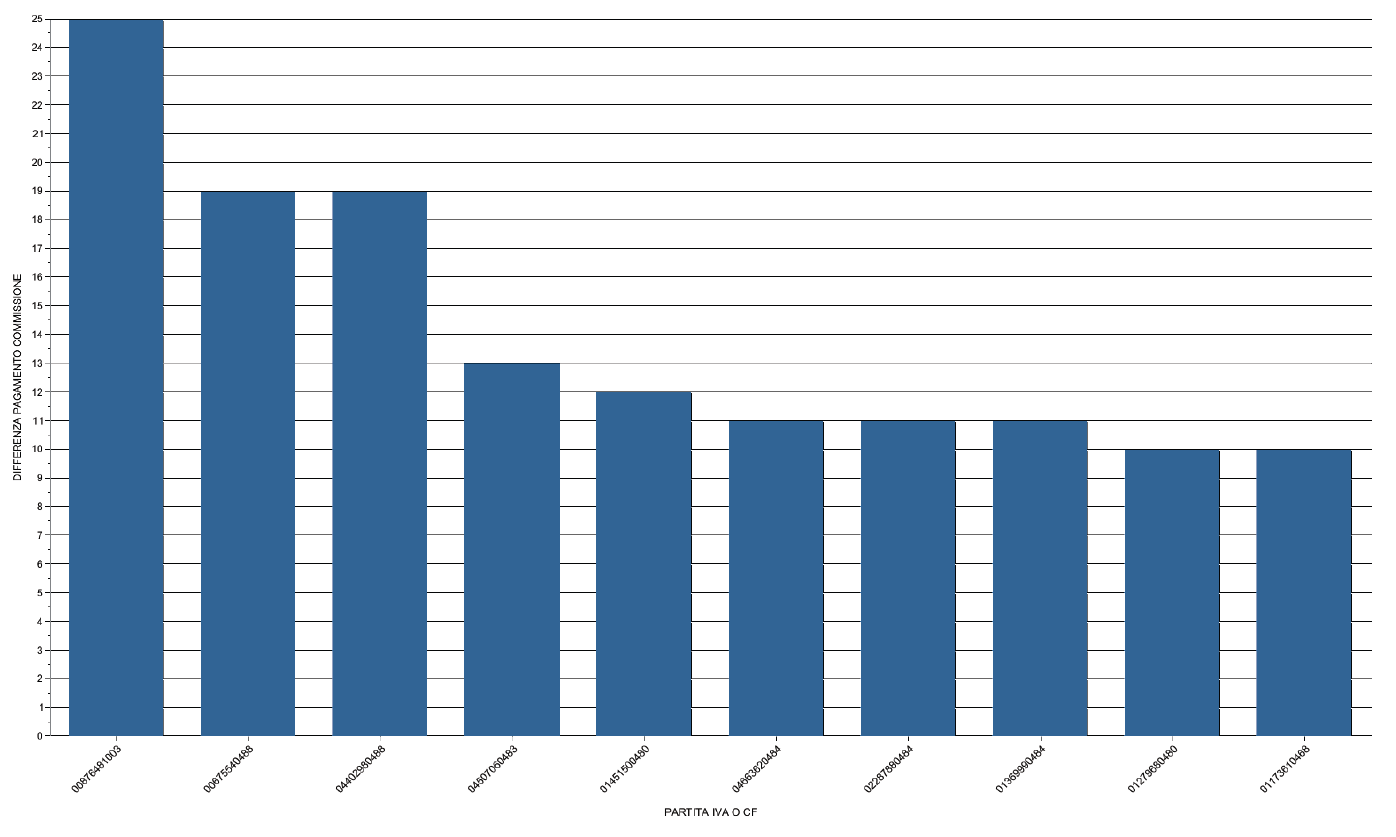
\includegraphics[scale=0.5]{top10_differenzepagamento_aziende.png}
			\caption{TOP 10 Anni di Pagamento per Aziende, grafico.}
			\label{fig:top10_differenzepagamento_aziende}
		\end{figure}
		
		\begin{figure}[h!]
			\centering
				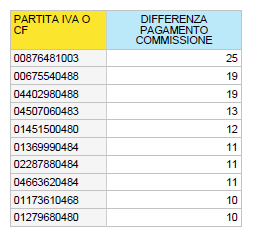
\includegraphics[scale=0.8]{top10_differenzepagamento_aziende_tab.png}
			\caption{TOP 10 Anni di Pagamento per Aziende, tabella.}
			\label{fig:top10_differenzepagamento_aziende_tab}
		\end{figure}
		
		\begin{figure}[h!]
			\centering
				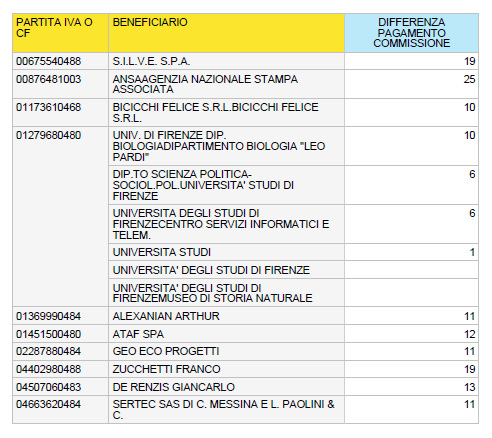
\includegraphics[scale=0.8]{top10_differenzepagamento_aziende_tab_dis.png}
			\caption{TOP 10 Anni di Pagamento per Aziende, tabella disaggregata.}
			\label{fig:top10_differenzepagamento_aziende_tab_dis}
		\end{figure}
		
		Al primo posto, con un lavoro durato ben 25 anni, troviamo l'\textit{ANSA} (\textit{Agenzia Nazionale Stampa Associata}), mentre al secondo e terzo posto, a pari merito con 19 anni, troviamo l'Azienda \textit{S.I.L.V.E. s.p.a.}, che si occupa di impianti di illuminazione elettrica, ed l'Azienda \textit{Zucchetti Franco}, i cui servizi ci sono ignoti. Le altre commissioni presenti in questa Top-10 vano invece dai 13 ai 10 anni di durata.
		
		\FloatBarrier
		
	\section{Analisi per tipo di Atto di Impegno} \label{sec:tipo_atto_impegno}
		
		Concludiamo questa serie di analisi con alcune osservazioni riguardanti il tipo di Atto di Impegno indicato per ogni commissione, ovvero sul campo \texttt{TIPO\_ATTO\_IMPEGNO} del nostro file \texttt{.csv}.\\
		Il tipo di Atto di Impegno è una sigla, di due o tre lettere, che indica con quale priorità è stato commissionato un certo mandato, ovvero l'importanza attribuita ad ogni commissione. A parte sigle poco utilizzate o deprecate, le due più importanti in questo senso sono \textit{DD} e \textit{CC}, che stanno, rispettivamente, per \textit{Decreto} (o \textit{Determina}) \textit{Dirigenziale} e per \textit{Consiglio Comunale}.\\
		Un \textit{Decreto Dirigenziale} indicherà quindi tutte quelle decisioni prese da un dirigente del settore (solitamente il dirigente della Direzione di Servizio che commissiona il lavoro), che non necessitano consiglio o approvazione da parte di altri settori; al contrario, un lavoro commissionato dal \textit{Consiglio Comunale} sarà sicuramente un lavoro molto più importante o impegnativo, in quanto richiede che tutto il Consiglio Comunale sia d'accordo sui dettagli e le modalità di quel particolare mandato.
		
		\subsection{\textit{Consigli Comunali} negli anni} \label{subsec:cc_negli_anni}
		
			Una prima, semplice analisi in questo senso può essere la determinazione di quanti mandati sono stati commissionati dal Consiglio Comunale negli anni, per capire in quale anno sono state prese più ``decisioni importanti''.\\
			Effettuiamo quindi un'analisi su due dimensioni: il tipo di Atto d'Impegno, che sarà fissato su \textit{CC}, e l'Anno di Commissione, che spazierà sull'intero dominio.\\
			
			\begin{figure}[h!]
				\centering
					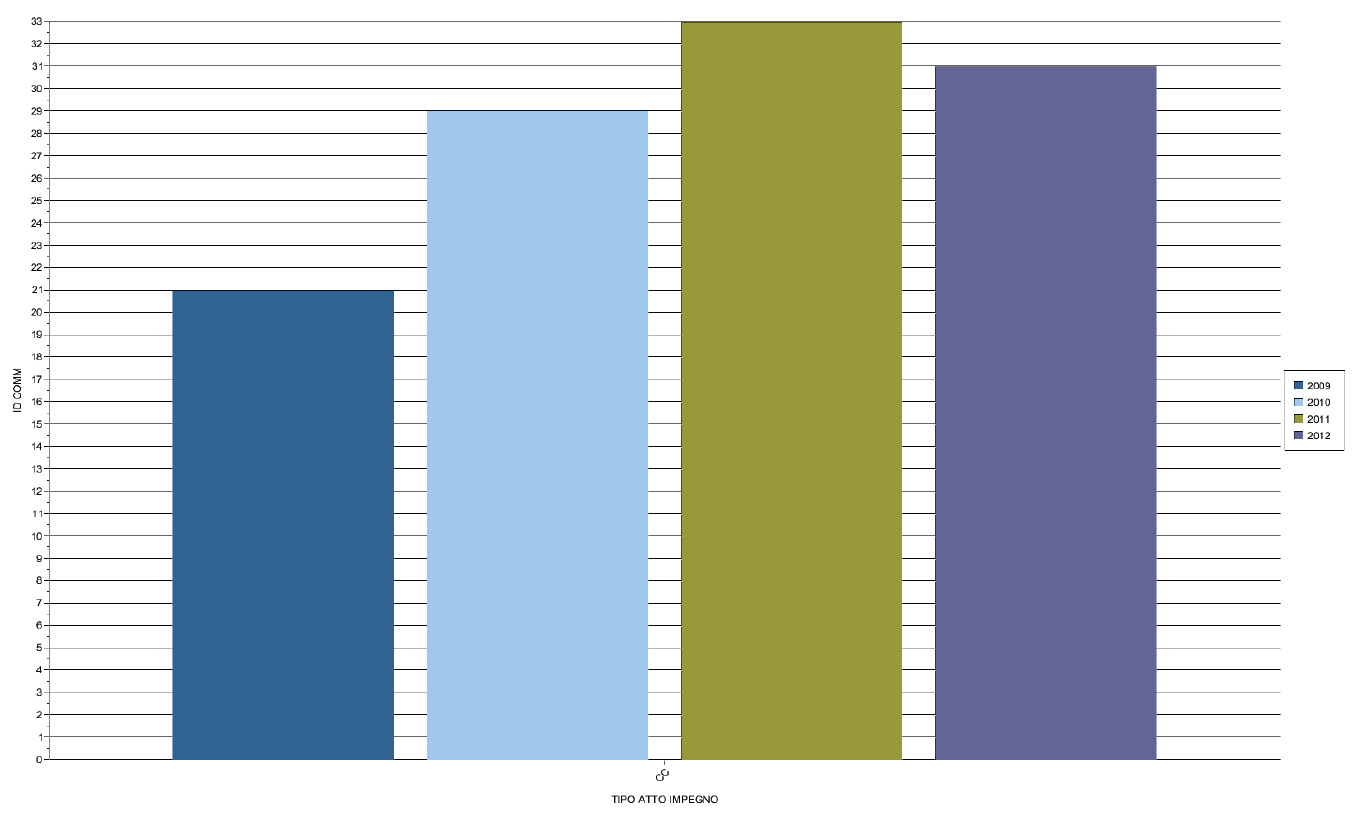
\includegraphics[scale=0.5]{cc_2009-2013.png}
				\caption{\textit{Consigli Comunali} negli anni, grafico.}
				\label{fig:cc_2009-2013}
			\end{figure}
			
			\begin{figure}[h!]
				\centering
					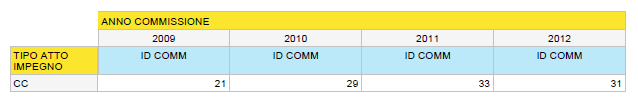
\includegraphics[scale=0.8]{cc_2009-2013_tab.png}
				\caption{\textit{Consigli Comunali} negli anni, tabella.}
				\label{fig:cc_2009-2013_tab}
			\end{figure}
			
			Si osserva innanzitutto che prima del 2009 non è stato fatto (o più ragionevolmente, non è stato registrato) alcun \textit{Consiglio Comunale}, come anche nel 2013. Quindi per quanto riguarda gli anni che vanno dal 2009 al 2012, si vede che la differenza tra i vari anni è minima, raggiungendo un picco nel 2011, con 33 \textit{Consigli Comunali}.
			
			\FloatBarrier
			
		\subsection{Confronto: CC-DD nel 2009-2013} \label{subsec:cc-dd_2009-2013}
		
			Volendo entrare adesso più nel dettaglio rispetto all'analisi precedente, possiamo includere anche il numero, per ogni anno, di lavori approvati per \textit{Decreto Dirigenziale}, mettendo in relazione quanti lavori sono stati commissionati per \textit{Consiglio Comunale} e quanti per \textit{Decreto Dirigenziale}.\\
			
			\begin{figure}[h!]
				\centering
					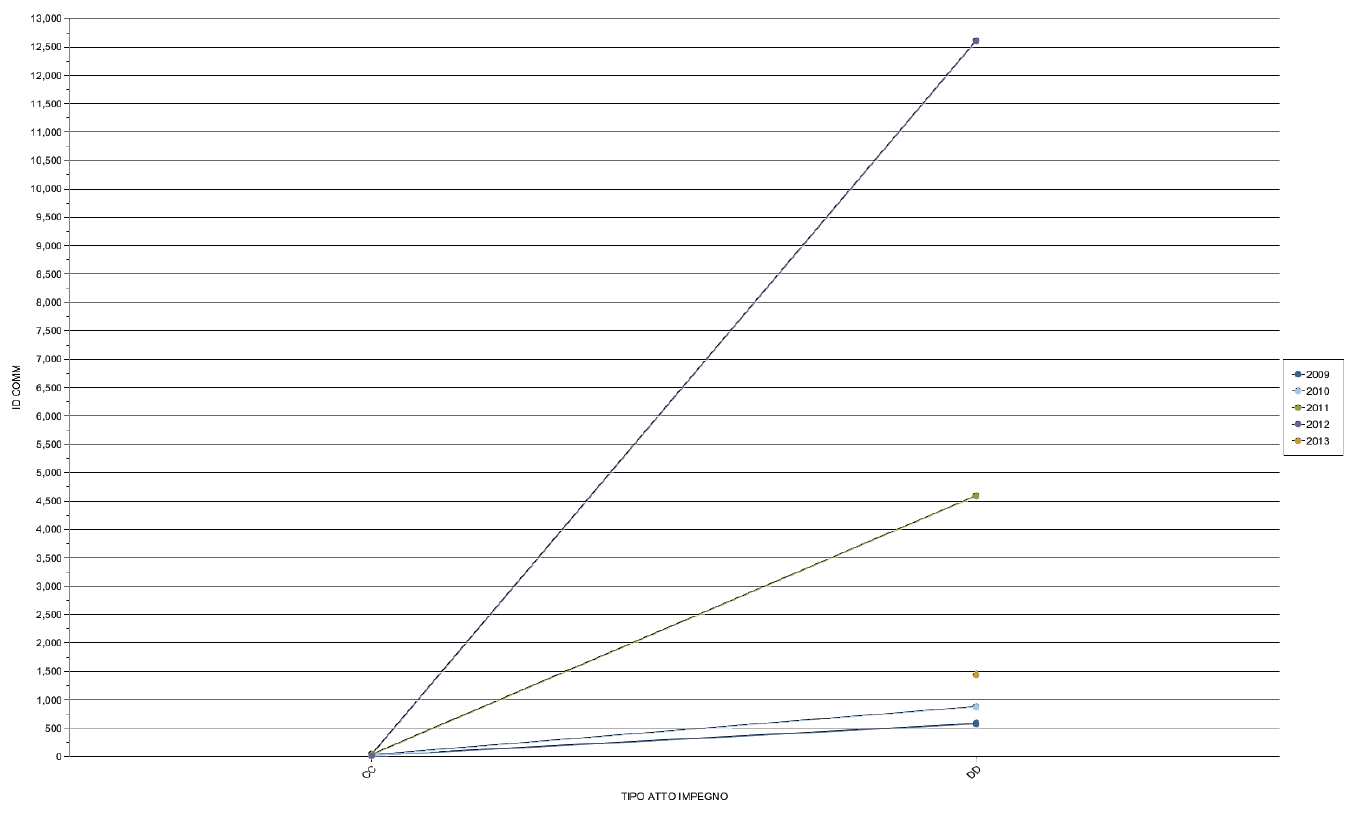
\includegraphics[scale=0.5]{cc-dd_2009-2013_a.png}
				\caption{\textit{Consigli Comunali} e \textit{Decreti Dirigenziali} negli anni, grafico a linee.}
				\label{fig:cc-dd_2009-2013_a}
			\end{figure}
			
			\begin{figure}[h!]
				\centering
					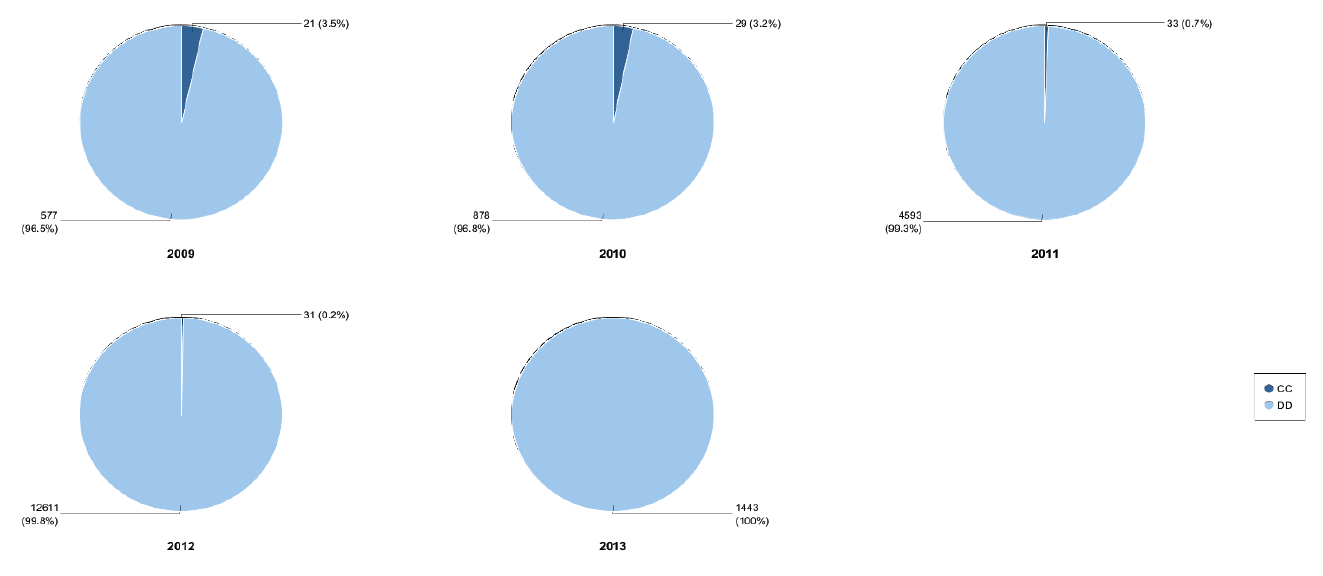
\includegraphics[scale=0.5]{cc-dd_2009-2013_b.png}
				\caption{\textit{Consigli Comunali} e \textit{Decreti Dirigenziali} negli anni, grafici a torta.}
				\label{fig:cc-dd_2009-2013_b}
			\end{figure}
			
			\begin{figure}[h!]
				\centering
					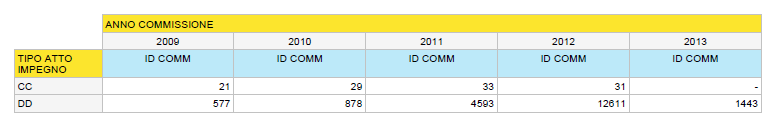
\includegraphics[scale=0.8]{cc-dd_2009-2013_tab.png}
				\caption{\textit{Consigli Comunali} e \textit{Decreti Dirigenziali} negli anni, tabella.}
				\label{fig:cc-dd_2009-2013_tab}
			\end{figure}
			
			Come ci si poteva aspettare, i \textit{Decreti Dirigenziali}, associati a lavori più semplici o meno importanti, sono molti di più rispetto ai \textit{Consigli Comunali}, come possiamo vedere sia dai grafici che dalla tabella. Inoltre, se osserviamo i grafici a torta in Figura \ref{fig:cc-dd_2009-2013_b}, si nota anche che in percentuale i \textit{Consigli Comunali} sono andati a diminuire negli anni rispetto ai \textit{Decreti Dirigenziali}. Escludendo motivi tecnici del settore (sui quali non possiamo fare speculazioni di alcun tipo), una possibile spiegazione potrebbe essere che, essendo i \textit{Consigli Comunali} molto più importanti di un qualsiasi \textit{Decreto Dirigenziale}, questi sono stati tracciati e registrati in modo più accurato e preciso rispetto ai \textit{Decreti Dirigenziali}, che molto probabilmente venivano persi tra le scartoffie e la burocrazia del Comune, almeno fino al Decreto Sviluppo 2012.
			
			\FloatBarrier